% Suggested filename: סיכום_יסודות_החשמל.tex
\documentclass[12pt]{article}

%========== (1) Math Packages ==========
\usepackage{amsmath,amssymb,amsthm}

%========== (2) General Packages: Hebrew support, fonts, etc ==========
\usepackage{xcolor}
\usepackage{float}
\usepackage{graphicx}
\usepackage{hyperref}
\usepackage{booktabs}
\usepackage{enumerate}
\usepackage{fancyvrb}
\usepackage{fancyhdr}
\usepackage{setspace}
\usepackage[most]{tcolorbox}

\usepackage{fontspec}
\usepackage{polyglossia}

\newcommand{\enquote}[1]{\textquotedblleft #1\textquotedblright}

% Language settings
\setdefaultlanguage{hebrew}
\setotherlanguage{english}

% Fonts
% Using David CLM as requested, ensure it's installed on the system
\newfontfamily\hebrewfont[Script=Hebrew]{David CLM}
\newfontfamily\englishfont{Times New Roman}
\newfontfamily\hebrewfonttt[Script=Hebrew]{David CLM} % Often monospaced fonts are needed for tt, but David CLM for consistency

% Hyperref link color settings
\hypersetup{
  colorlinks=true,
  linkcolor=black,
  urlcolor=black,
  citecolor=black
}

%========== Spacing and Paragraphs ==========
\onehalfspacing
\setlength{\parskip}{6pt}
\setlength{\parindent}{0pt}

%========== Header/Footer Settings ==========
\pagestyle{fancy}
\setlength{\headheight}{14.5pt}
\addtolength{\topmargin}{-2.5pt}
\fancyhf{}
\lhead{} % Left header empty or can add title later
\rhead{\today} % Right header shows today's date
\cfoot{\thepage} % Center footer shows page number

%========== tcolorbox Setup ==========
% Re-defining based on the user's explicit definitions block
\tcbset{
  boxsep=5pt,
  top=5pt, bottom=5pt, left=5pt, right=5pt,
  middle=5pt,
  sharp corners, % Added based on the specific box definitions below
  enhanced       % Added based on the specific box definitions below
}

%========== Special Boxes: Definition, Remark, Example ==========
% Using slightly less pale backgrounds but still soft, and frames as specified.
% Re-defining based on the user's explicit definitions block
\newtcolorbox{definitionBox}[1]{
  title=#1,
  colback=green!5!white, % Slightly more saturated than 1!white
  colframe=green!50!black,
  sharp corners,
  enhanced
}

\newtcolorbox{remarkBox}[1]{
  title=#1,
  colback=yellow!5!white, % Slightly more saturated
  colframe=yellow!50!black,
  sharp corners,
  enhanced
}

\newtcolorbox{exampleBox}[1]{
  title=#1,
  colback=red!5!white, % Slightly more saturated
  colframe=red!50!black,
  sharp corners,
  enhanced
}

% Custom box for Laws/Principles, using the blue specified in the generic tcbset
\newtcolorbox{lawBox}[1]{
  title=#1,
  colback=blue!5!white, % Slightly more saturated
  colframe=blue!50!black,
  sharp corners,
  enhanced
}


% Bullet fix
\renewcommand{\labelitemi}{$\bullet$} % Changed to a standard bullet

% Table of contents setup (as provided)
\usepackage{tocloft}
\usepackage{etoolbox}

\makeatletter
\renewcommand\tableofcontents{\section*{ \contentsname}
    @starttoc{toc}}
\makeatother

\begin{document}

\begin{center}
    \Large\bfseries סיכום מקיף ביסודות החשמל לתלמידי תיכון
\end{center}

\vspace{1em} % Add some space after the title

\tableofcontents

\newpage % Start the first section on a new page

\section{מטען חשמלי וחוק קולון}

\begin{definitionBox}{הגדרה: מטען חשמלי}
מטען חשמלי הוא תכונה יסודית של חלקיקים מסוימים, כמו אלקטרונים ופרוטונים, הגורמת להם להפעיל כוח חשמלי זה על זה. מטען חשמלי יכול להיות חיובי (+) או שלילי (-). יחידת המטען הבסיסית נקראת \enquote{אלמנטרית} וסימונה \(e\). גופים ניטרליים חשמלית הם בעלי כמות שווה של מטענים חיוביים ושליליים.
\end{definitionBox}

\begin{remarkBox}{הערה: שימור מטען}
חוק שימור המטען קובע שמטען חשמלי אינו נוצר יש מאין ואינו נעלם יש מאין. בסך הכל, המטען החשמלי הכולל במערכת מבודדת נשאר קבוע.
\end{remarkBox}

כאשר גופים טעונים מתקרבים זה לזה, פועל ביניהם כוח חשמלי. כוח זה נקרא גם כוח קולון, והוא יכול להיות כוח משיכה (בין מטענים שונים, + ל-) או כוח דחייה (בין מטענים זהים, + ל+ או - ל-). עוצמת כוח זה מתוארת על ידי חוק קולון.

\begin{lawBox}{חוק קולון}
חוק קולון מתאר את עוצמת הכוח החשמלי הפועל בין שני מטענים נקודתיים \(q_1\) ו-\(q_2\), המופרדים על ידי מרחק \(r\). החוק קובע שהכוח יחסי ישר למכפלת גודלי המטענים ויחסי הפוך לריבוע המרחק ביניהם.
בצורה מתמטית, עוצמת הכוח \(F\) נתונה על ידי הנוסחה:
\begin{equation*}
F = k \frac{|q_1 q_2|}{r^2}
\end{equation*}
כאשר \(k\) הוא קבוע קולון, שערכו בריק הוא בערך \(8.988 \times 10^9 \, \text{N} \cdot \text{m}^2/\text{C}^2\).
\end{lawBox}

חשוב להבין שחוק קולון מתייחס לגודל הכוח. כיוון הכוח הוא לאורך הקו המחבר את שני המטענים. אם המטענים זהים (שניהם חיוביים או שניהם שליליים), הכוח הוא כוח דחייה (החוצה מהקו המחבר). אם המטענים שונים (אחד חיובי ואחד שלילי), הכוח הוא כוח משיכה (פנימה לאורך הקו המחבר).

\begin{figure}[H]
  \centering
  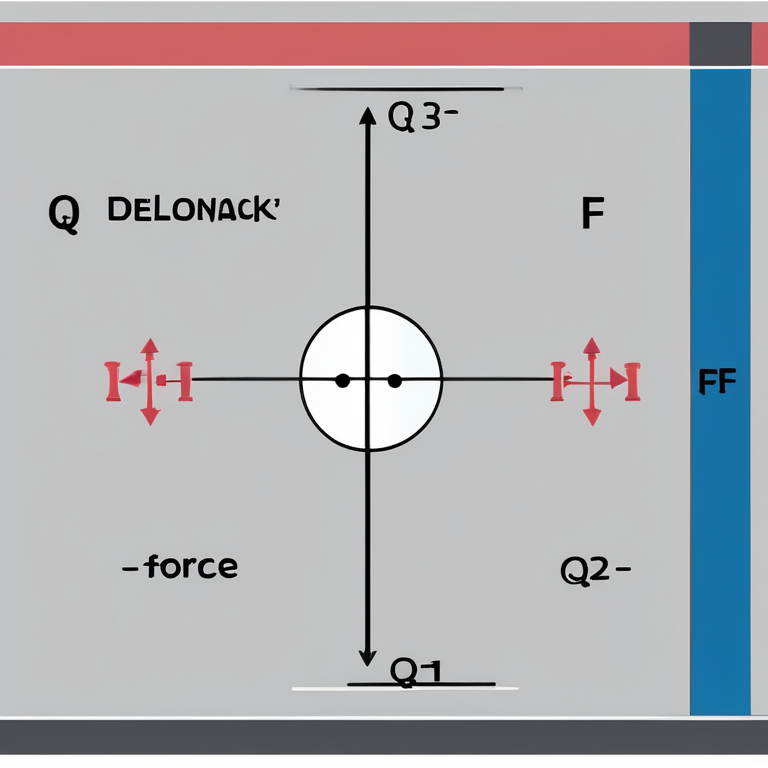
\includegraphics[width=0.6\textwidth]{files/coulomb_law_diagram.png}
  \caption{דיאגרמה להמחשת חוק קולון בין שני מטענים נקודתיים.}
\end{figure}

\begin{exampleBox}{דוגמה: חישוב כוח קולון}
נניח שיש לנו שני מטענים נקודתיים: \(q_1 = +2 \times 10^{-9} \, \text{C}\) ו-\(q_2 = -3 \times 10^{-9} \, \text{C}\). המרחק ביניהם הוא \(r = 0.05 \, \text{m}\). מהו גודל הכוח החשמלי הפועל ביניהם, ומה כיוונו?

נשתמש בנוסחת חוק קולון:
\[F = k \frac{|q_1 q_2|}{r^2}\]
נציב את הערכים:
\[F = (8.988 \times 10^9 \, \text{N} \cdot \text{m}^2/\text{C}^2) \frac{|(+2 \times 10^{-9} \, \text{C})(-3 \times 10^{-9} \, \text{C})|}{(0.05 \, \text{m})^2}\]
\[F = (8.988 \times 10^9) \frac{6 \times 10^{-18}}{0.0025}\]
\[F = (8.988 \times 10^9) \times (2.4 \times 10^{-15})\]
\[F \approx 21.57 \times 10^{-6} \, \text{N}\]
גודל הכוח הוא בערך \(21.57\) מיקרו-ניוטון.
מכיוון שהמטענים הם בעלי סימן שונה (חיובי ושלילי), הכוח הוא כוח משיכה. כל מטען מושך את השני אליו.
\end{exampleBox}

עבור מערכת של יותר משני מטענים, הכוח הכולל הפועל על מטען מסוים הוא סכום וקטורי של כוחות קולון הפועלים עליו מכל אחד מהמטענים האחרים. זהו עקרון הסופרפוזיציה.
(הערה: בתגובה הקודמת התבקש להסביר את עקרון הסופרפוזיציה בקצרה - זהו ההסבר הבסיסי שלו).
\begin{remarkBox}{הערה: עקרון הסופרפוזיציה}
כאשר על מטען נקודתי פועלים כוחות מכמה מטענים אחרים, הכוח השקול הפועל עליו הוא הסכום הווקטורי של כל הכוחות הפועלים בנפרד. לדוגמה, אם מטענים \(q_2, q_3, \dots\) מפעילים כוחות \( \vec{F}_{12}, \vec{F}_{13}, \dots \) על מטען \(q_1\), אזי הכוח הכולל על \(q_1\) הוא \( \vec{F}_{1, \text{total}} = \vec{F}_{12} + \vec{F}_{13} + \dots \).
\end{remarkBox}

\section{שדה חשמלי וקווי שדה}

מושג השדה החשמלי נוצר כדי לתאר את ההשפעה של מטען על המרחב סביבו, גם לפני שמטען אחר נמצא שם. השדה החשמלי הוא למעשה תכונה של המרחב הנוצרת על ידי מטענים.

\begin{definitionBox}{הגדרה: שדה חשמלי}
השדה החשמלי (\(\vec{E}\)) בנקודה מסוימת במרחב מוגדר ככוח החשמלי (\(\vec{F}\)) שיפעל על מטען בוחן חיובי קטן (\(q_0\)) המוצב בנקודה זו, מחולק בגודל מטען הבוחן:
\begin{equation*}
\vec{E} = \frac{\vec{F}}{q_0}
\end{equation*}
יחידות השדה החשמלי במערכת היחידות הבינלאומית (SI) הן ניוטון לקולון (\(\text{N}/\text{C}\)) או, באופן שקול, וולט למטר (\(\text{V}/\text{m}\)).
\end{definitionBox}

השדה החשמלי הוא גודל וקטורי, בעל גודל וכיוון בכל נקודה במרחב. כיוון השדה החשמלי בנקודה מסוימת מוגדר ככיוון הכוח שיפעל על מטען חיובי המוצב באותה נקודה. לכן, השדה מתרחק ממטענים חיוביים ומתקרב למטענים שליליים.

עוצמת השדה החשמלי במרחק \(r\) ממטען נקודתי \(q\) נתונה על ידי:
\begin{equation*}
E = k \frac{|q|}{r^2}
\end{equation*}
כיוון השדה הוא רדיאלי החוצה עבור מטען חיובי, ורדיאלי פנימה עבור מטען שלילי.

כדי לדמיין את השדה החשמלי, משתמשים במושג \enquote{קווי שדה}.

\begin{definitionBox}{הגדרה: קווי שדה חשמלי}
קווי שדה חשמלי הם קווים דמיוניים שמשרטטים במרחב כדי להמחיש את השדה. לכל קו שדה יש כיוון, והוא מצביע על כיוון השדה החשמלי בנקודה זו. התכונות העיקריות של קווי השדה הן:
\begin{itemize}
    \item הם יוצאים ממטענים חיוביים ונכנסים למטענים שליליים.
    \item צפיפות קווי השדה בנקודה מסוימת מעידה על עוצמת השדה החשמלי באותה נקודה (ככל שהקווים צפופים יותר, השדה חזק יותר).
    \item קווי שדה אינם יכולים לחצות זה את זה (מכיוון שבכל נקודה במרחב יש כיוון שדה יחיד).
\end{itemize}
\end{definitionBox}

\begin{figure}[H]
  \centering
  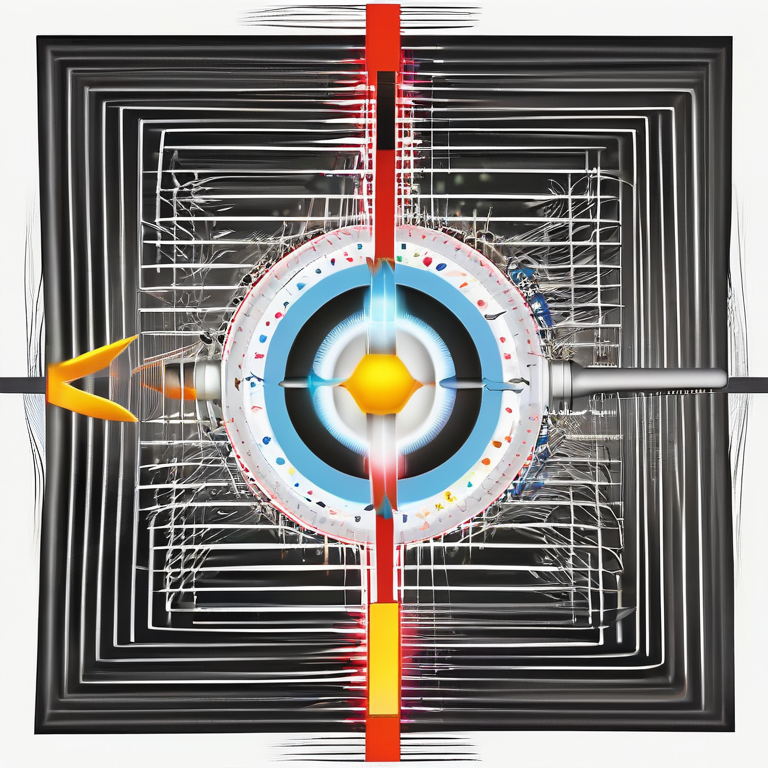
\includegraphics[width=0.6\textwidth]{files/electric_field_diagram.png}
  \caption{דיאגרמה להמחשת קווי שדה חשמלי סביב מטען נקודתי חיובי ושלילי, ובין שני מטענים שונים.}
\end{figure}

\begin{exampleBox}{דוגמה: שדה חשמלי ממטען נקודתי}
מהו גודל השדה החשמלי במרחק של \(10 \, \text{cm}\) ממטען נקודתי של \(+5 \times 10^{-9} \, \text{C}\)? מה כיוון השדה?

המרחק הוא \(r = 10 \, \text{cm} = 0.1 \, \text{m}\). גודל המטען הוא \(q = +5 \times 10^{-9} \, \text{C}\).
נשתמש בנוסחה לעוצמת השדה החשמלי ממטען נקודתי:
\[E = k \frac{|q|}{r^2}\]
\[E = (8.988 \times 10^9 \, \text{N} \cdot \text{m}^2/\text{C}^2) \frac{5 \times 10^{-9} \, \text{C}}{(0.1 \, \text{m})^2}\]
\[E = (8.988 \times 10^9) \frac{5 \times 10^{-9}}{0.01}\]
\[E = (8.988 \times 10^9) \times (500 \times 10^{-9})\]
\[E = 8.988 \times 500 \, \text{N}/\text{C}\]
\[E \approx 4494 \, \text{N}/\text{C}\]
גודל השדה החשמלי הוא בערך \(4494 \, \text{N}/\text{C}\). מכיוון שהמטען חיובי, כיוון השדה בנקודה זו הוא רדיאלי החוצה מהמטען.
\end{exampleBox}

עקרון הסופרפוזיציה חל גם על שדות חשמליים: השדה החשמלי הכולל בנקודה מסוימת הנוצר על ידי מספר מטענים הוא הסכום הווקטורי של השדות החשמליים שכל מטען היה יוצר בנפרד באותה נקודה.

\section{פוטנציאל חשמלי ומתח}

פוטנציאל חשמלי ומתח חשמלי קשורים לאנרגיה פוטנציאלית חשמלית, בדומה לקשר בין שדה חשמלי וכוח חשמלי. בעוד שהשדה והכוח הם וקטורים, הפוטנציאל והמתח הם סקלרים, מה שהופך אותם לעיתים קלים יותר לחישוב.

\begin{definitionBox}{הגדרה: אנרגיה פוטנציאלית חשמלית}
אנרגיה פוטנציאלית חשמלית (\(U\)) היא האנרגיה האגורה במערכת של מטענים כתוצאה ממיקומם היחסי זה לזה בשדה חשמלי. העבודה שמבצע הכוח החשמלי להזיז מטען מנקודה אחת לאחרת שווה לשינוי השלילי באנרגיה הפוטנציאלית החשמלית.
\end{definitionBox}

בדומה לשדה החשמלי, המוגדר ככוח ליחידת מטען, הפוטנציאל החשמלי מוגדר כאנרגיה פוטנציאלית חשמלית ליחידת מטען.

\begin{definitionBox}{הגדרה: פוטנציאל חשמלי}
הפוטנציאל החשמלי (\(V\)) בנקודה מסוימת במרחב הוא האנרגיה הפוטנציאלית החשמלית (\(U\)) ליחידת מטען בוחן חיובי המוצב בנקודה זו:
\begin{equation*}
V = \frac{U}{q_0}
\end{equation*}
יחידת הפוטנציאל החשמלי היא ג'ול לקולון (\(\text{J}/\text{C}\)), הנקראת וולט (\(\text{V}\)).
\end{definitionBox}

לרוב, מה שמעניין יותר הוא \enquote{הפרש הפוטנציאלים} בין שתי נקודות, המכונה \enquote{מתח חשמלי}.

\begin{definitionBox}{הגדרה: מתח חשמלי (הפרש פוטנציאלים)}
המתח החשמלי (\(\Delta V\)) בין שתי נקודות A ו-B הוא הפרש הפוטנציאלים החשמליים בין הנקודות הללו:
\begin{equation*}
\Delta V = V_B - V_A = \frac{\Delta U}{q_0}
\end{equation*}
המתח החשמלי שווה לעבודה (\(W\)) שיש לבצע ללא שינוי באנרגיה הקינטית כדי להזיז מטען בוחן חיובי קטן מנקודה A לנקודה B, מחולקת בגודל מטען הבוחן:
\begin{equation*}
\Delta V = \frac{W_{A \to B}}{q_0}
\end{equation*}
גם יחידת המתח היא וולט (\(\text{V}\)). המתח הוא הכוח המניע מטענים לנוע במעגל חשמלי.
\end{definitionBox}

\begin{remarkBox}{הערה: פוטנציאל ממטען נקודתי}
הפוטנציאל החשמלי במרחק \(r\) ממטען נקודתי \(q\) (ביחס לאינסוף, שם הפוטנציאל מוגדר כאפס) נתון על ידי:
\[V = k \frac{q}{r}\]
שימו לב שזו כמות סקלרית, ולכן אין בה ערך מוחלט של המטען \(q\). מטענים חיוביים יוצרים פוטנציאל חיובי ומטענים שליליים יוצרים פוטנציאל שלילי.
\end{remarkBox}

\begin{exampleBox}{דוגמה: חישוב מתח}
כמה עבודה נדרשת כדי להזיז מטען של \(+4 \times 10^{-6} \, \text{C}\) מנקודה בעלת פוטנציאל \(V_A = 10 \, \text{V}\) לנקודה בעלת פוטנציאל \(V_B = 50 \, \text{V}\)?

השינוי בפוטנציאל (המתח) הוא \(\Delta V = V_B - V_A = 50 \, \text{V} - 10 \, \text{V} = 40 \, \text{V}\).
העבודה הנדרשת ניתנת על ידי \(W = q_0 \Delta V\).
נציב את הערכים:
\[W = (4 \times 10^{-6} \, \text{C}) \times (40 \, \text{V})\]
\[W = 160 \times 10^{-6} \, \text{J}\]
\[W = 1.6 \times 10^{-4} \, \text{J}\]
נדרשת עבודה של \(1.6 \times 10^{-4}\) ג'ול. עבודה חיובית פירושה שגורם חיצוני (לא הכוח החשמלי) ביצע עבודה זו.
\end{exampleBox}

\section{חוק אוהם והתנגדות חשמלית}

כאשר יש הפרש פוטנציאלים (מתח) בין שתי נקודות במוליך, נוצר זרם חשמלי - תנועה מסודרת של מטענים חשמליים. הקשר בין המתח, הזרם, ותכונה של המוליך הנקראת התנגדות חשמלית, מתואר על ידי חוק אוהם.

\begin{definitionBox}{הגדרה: זרם חשמלי}
זרם חשמלי (\(I\)) מוגדר כקצב מעבר מטען חשמלי דרך שטח חתך נתון במוליך.
\begin{equation*}
I = \frac{\Delta q}{\Delta t}
\end{equation*}
כאשר \(\Delta q\) הוא כמות המטען שעוברת דרך שטח החתך בזמן \(\Delta t\).
יחידת הזרם החשמלי היא קולון לשנייה (\(\text{C}/\text{s}\)), הנקראת אמפר (\(\text{A}\)). כיוון הזרם המוסכם הוא כיוון תנועת מטענים חיוביים, למרות שבאופן מעשי במתכות אלו בדרך כלל אלקטרונים (מטענים שליליים) שנעים בכיוון ההפוך.
\end{definitionBox}

\begin{definitionBox}{הגדרה: התנגדות חשמלית}
התנגדות חשמלית (\(R\)) היא מידה ליכולת של חומר להתנגד למעבר זרם חשמלי דרכו. חומרים בעלי התנגדות נמוכה נקראים מוליכים, וחומרים בעלי התנגדות גבוהה נקראים מבודדים. ההתנגדות של מוליך תלויה בחומר ממנו הוא עשוי (התנגדות סגולית), אורכו, שטח החתך שלו, ולעיתים גם בטמפרטורה.
\begin{equation*}
R = \rho \frac{L}{A}
\end{equation*}
כאשר \(\rho\) היא ההתנגדות הסגולית של החומר (יחידות אוהם-מטר, \(\Omega \cdot \text{m}\)), \(L\) הוא אורך המוליך, ו-\(A\) הוא שטח החתך שלו.
יחידת ההתנגדות היא וולט לאמפר (\(\text{V}/\text{A}\)), הנקראת אוהם (\(\Omega\)).
\end{definitionBox}

הקשר בין המתח, הזרם וההתנגדות במוליך או רכיב נקרא חוק אוהם.

\begin{lawBox}{חוק אוהם}
חוק אוהם קובע שבשביל חומרים מסוימים (חומרים אוהמיים), הזרם החשמלי (\(I\)) העובר דרך רכיב יחסי ישר למתח (\(V\)) המופעל עליו, והיחס קבוע ושווה להתנגדות (\(R\)) של הרכיב.
\begin{equation*}
V = I \cdot R
\end{equation*}
או, ניתן לבטא זאת גם כ- \(I = \frac{V}{R}\) או \(R = \frac{V}{I}\).
\end{lawBox}

\begin{figure}[H]
  \centering
  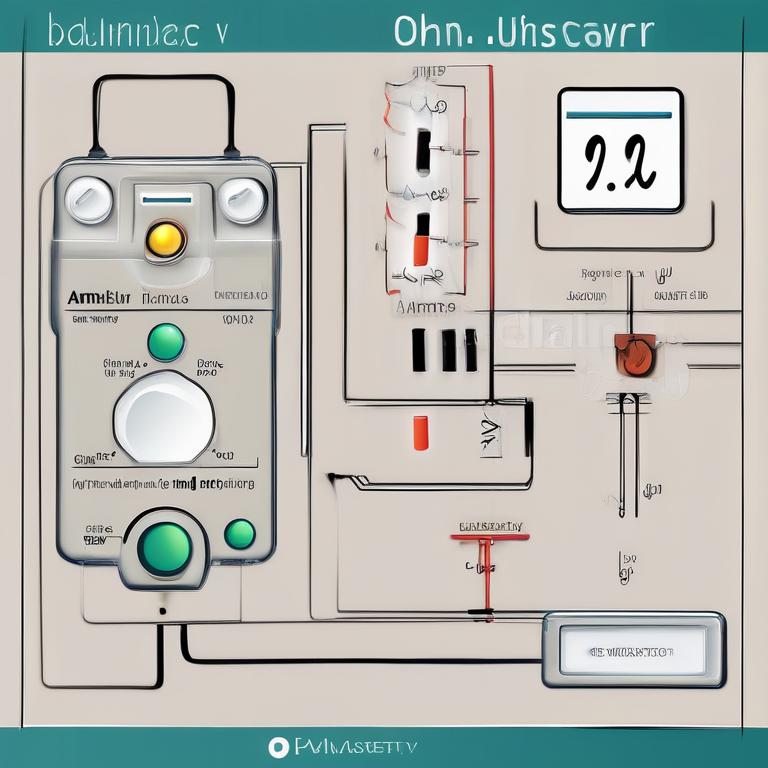
\includegraphics[width=0.6\textwidth]{files/ohms_law_circuit.png}
  \caption{דיאגרמה של מעגל חשמלי פשוט הממחישה את הקשר בין מתח (סוללה), זרם (מסומן על ידי חץ) והתנגדות (נגד).}
\end{figure}

\begin{remarkBox}{הערה: מגבלות חוק אוהם}
חוק אוהם אינו חוק יסוד של הטבע כמו חוק שימור האנרגיה. הוא תיאור אמפירי המתאים למגוון רחב של חומרים ורכיבים בתנאים מסוימים (לרוב טמפרטורה קבועה). חומרים שאינם מקיימים את חוק אוהם נקראים חומרים לא-אוהמיים (כמו דיודות וטרנזיסטורים).
\end{remarkBox}

\begin{exampleBox}{דוגמה: חישוב זרם}
למנורה יש התנגדות של \(240 \, \Omega\). מהו הזרם שיעבור דרכה כאשר היא מחוברת למתח של \(120 \, \text{V}\)?

נשתמש בחוק אוהם: \(V = I \cdot R\). נרצה לחשב את הזרם \(I\), לכן נסדר את הנוסחה: \(I = \frac{V}{R}\).
נציב את הערכים:
\[I = \frac{120 \, \text{V}}{240 \, \Omega}\]
\[I = 0.5 \, \text{A}\]
הזרם שיעבור דרך המנורה הוא \(0.5\) אמפר.
\end{exampleBox}

\section{מעגלים חשמליים (טורי ומקבילי)}

מעגל חשמלי הוא נתיב סגור שבו יכול לעבור זרם חשמלי. מעגלים פשוטים כוללים בדרך כלל מקור מתח (כמו סוללה), רכיבים (כמו נגדים, נורות), וחוטי חיבור. רכיבים במעגל יכולים להיות מחוברים בשני אופנים עיקריים: בטור או במקביל.

\begin{definitionBox}{הגדרה: מעגל חשמלי}
מעגל חשמלי הוא מסלול מוליך סגור המאפשר תנועת מטענים (זרם חשמלי), בדרך כלל כתוצאה מהפרש פוטנציאלים שמספק מקור כוח אלקטרו-מניע (כא"מ), כמו סוללה.
\end{definitionBox}

\begin{figure}[H]
  \centering
  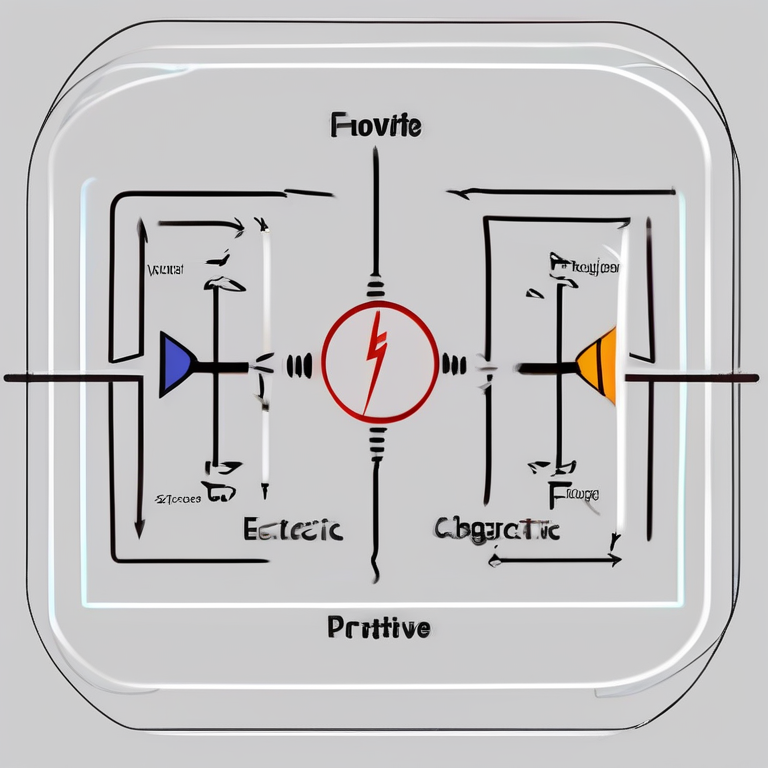
\includegraphics[width=0.6\textwidth]{files/simple_circuit_diagram.png}
  \caption{דיאגרמה של מעגל חשמלי פשוט הכולל סוללה, נגד ומפסק.}
\end{figure}

\subsection{מעגל טורי}
במעגל טורי, הרכיבים מחוברים זה אחר זה לאורך נתיב יחיד.

\begin{remarkBox}{מאפיינים של מעגל טורי}
\begin{itemize}
    \item \textbf{זרם:} הזרם שווה בכל נקודה במעגל הטורי. כל המטענים עוברים דרך כל רכיב ברציפות. \(I_{\text{total}} = I_1 = I_2 = I_3 = \dots\)
    \item \textbf{מתח:} המתח הכולל של מקור המתח מתחלק בין הרכיבים. סכום מפל המתחים על כל רכיב שווה למתח הכולל. \(V_{\text{total}} = V_1 + V_2 + V_3 + \dots\)
    \item \textbf{התנגדות שקולה:} ההתנגדות הכוללת (השקולה) של מעגל טורי שווה לסכום ההתנגדויות של כל הרכיבים. \(R_{\text{eq}} = R_1 + R_2 + R_3 + \dots\)
\end{itemize}
\end{remarkBox}

חישוב ההתנגדות השקולה במעגל טורי פשוט: מחברים את כל ההתנגדויות.

\begin{exampleBox}{דוגמה: מעגל טורי}
שני נגדים, \(R_1 = 10 \, \Omega\) ו-\(R_2 = 20 \, \Omega\), מחוברים בטור לסוללה של \(12 \, \text{V}\).
מהי ההתנגדות השקולה של המעגל?
\[R_{\text{eq}} = R_1 + R_2 = 10 \, \Omega + 20 \, \Omega = 30 \, \Omega\]
מהו הזרם הכולל במעגל? (נשתמש בחוק אוהם למעגל כולו)
\[I_{\text{total}} = \frac{V_{\text{total}}}{R_{\text{eq}}} = \frac{12 \, \text{V}}{30 \, \Omega} = 0.4 \, \text{A}\]
מכיוון שזה מעגל טורי, הזרם דרך כל נגד הוא \(0.4 \, \text{A}\).
מהו מפל המתח על כל נגד? (נשתמש בחוק אוהם לכל נגד בנפרד)
\[V_1 = I_1 \cdot R_1 = 0.4 \, \text{A} \times 10 \, \Omega = 4 \, \text{V}\]
\[V_2 = I_2 \cdot R_2 = 0.4 \, \text{A} \times 20 \, \Omega = 8 \, \text{V}\]
נבדוק: \(V_1 + V_2 = 4 \, \text{V} + 8 \, \text{V} = 12 \, \text{V}\), וזה אכן שווה למתח הכולל.
\end{exampleBox}

\subsection{מעגל מקבילי}
במעגל מקבילי, הרכיבים מחוברים דרך שני צמתים משותפים, כך שהזרם מתפצל בין הנתיבים השונים.

\begin{remarkBox}{מאפיינים של מעגל מקבילי}
\begin{itemize}
    \item \textbf{מתח:} המתח על כל רכיב המחובר במקביל שווה למתח הכולל של מקור המתח (בהנחה שאין התנגדות בחוטים). \(V_{\text{total}} = V_1 = V_2 = V_3 = \dots\)
    \item \textbf{זרם:} הזרם הכולל היוצא ממקור המתח מתפצל בין הנתיבים המקביליים. סכום הזרמים דרך כל נתיב שווה לזרם הכולל (חוק הצמתים של קירכהוף). \(I_{\text{total}} = I_1 + I_2 + I_3 + \dots\)
    \item \textbf{התנגדות שקולה:} היפוך ההתנגדות הכוללת (השקולה) של מעגל מקבילי שווה לסכום היפוכים ההתנגדויות של כל הרכיבים. \(\frac{1}{R_{\text{eq}}} = \frac{1}{R_1} + \frac{1}{R_2} + \frac{1}{R_3} + \dots\)
\end{itemize}
\end{remarkBox}

חישוב ההתנגדות השקולה במעגל מקבילי מסובך יותר. עבור שני נגדים במקביל, הנוסחה המפושטת היא \(R_{\text{eq}} = \frac{R_1 R_2}{R_1 + R_2}\). עבור יותר רכיבים, יש להשתמש בנוסחת הסכום של ההיפוכים. ההתנגדות השקולה במעגל מקבילי תמיד קטנה מההתנגדות הנמוכה ביותר במקביל.

\begin{exampleBox}{דוגמה: מעגל מקבילי}
שני נגדים, \(R_1 = 10 \, \Omega\) ו-\(R_2 = 20 \, \Omega\), מחוברים במקביל לסוללה של \(12 \, \text{V}\).
מהי ההתנגדות השקולה של המעגל?
\[\frac{1}{R_{\text{eq}}} = \frac{1}{R_1} + \frac{1}{R_2} = \frac{1}{10 \, \Omega} + \frac{1}{20 \, \Omega} = \frac{2}{20 \, \Omega} + \frac{1}{20 \, \Omega} = \frac{3}{20 \, \Omega}\]
\[R_{\text{eq}} = \frac{20}{3} \, \Omega \approx 6.67 \, \Omega\]
שימו לב שההתנגדות השקולה (\(6.67 \, \Omega\)) קטנה מההתנגדות הנמוכה ביותר (\(10 \, \Omega\)), כצפוי.
מהו המתח על כל נגד?
\[V_1 = V_2 = V_{\text{total}} = 12 \, \text{V}\]
מהו הזרם דרך כל נגד?
\[I_1 = \frac{V_1}{R_1} = \frac{12 \, \text{V}}{10 \, \Omega} = 1.2 \, \text{A}\]
\[I_2 = \frac{V_2}{R_2} = \frac{12 \, \text{V}}{20 \, \Omega} = 0.6 \, \text{A}\]
מהו הזרם הכולל במעגל? (סכום הזרמים דרך הענפים)
\[I_{\text{total}} = I_1 + I_2 = 1.2 \, \text{A} + 0.6 \, \text{A} = 1.8 \, \text{A}\]
נבדוק בחוק אוהם עם ההתנגדות השקולה: \(I_{\text{total}} = \frac{V_{\text{total}}}{R_{\text{eq}}} = \frac{12 \, \text{V}}{20/3 \, \Omega} = 12 \times \frac{3}{20} \, \text{A} = \frac{36}{20} \, \text{A} = 1.8 \, \text{A}\). התוצאות מתאימות.
\end{exampleBox}

\section{אלקטרומגנטיות וחוק פאראדיי}

אלקטרומגנטיות היא תחום בפיזיקה המאחד את תופעות החשמל והמגנטיות. מסתבר ששדות חשמליים משתנים יכולים ליצור שדות מגנטיים, ושדות מגנטיים משתנים יכולים ליצור שדות חשמליים (או ליתר דיוק, כוח אלקטרו-מניע שגורם לזרם). קשר זה הוא הבסיס לתופעות רבות כמו פעולת מנועים חשמליים וגנרטורים, ותופעות האור עצמן (שדה אלקטרומגנטי מתפשט).

\begin{remarkBox}{קשר בסיסי בין חשמל למגנטיות}
\begin{itemize}
    \item מטען חשמלי נייח יוצר שדה חשמלי.
    \item מטען חשמלי נע (זרם חשמלי) יוצר שדה מגנטי.
    \item שדה מגנטי משתנה בזמן משרה כוח אלקטרו-מניע (מתח) במוליך (אינדוקציה אלקטרומגנטית).
    \item שדה חשמלי משתנה בזמן יוצר שדה מגנטי.
\end{itemize}
\end{remarkBox}

אחד החוקים החשובים ביותר בתחום זה, המתאר כיצד שדה מגנטי משתנה יוצר מתח, הוא חוק פאראדיי לאינדוקציה אלקטרומגנטית.

\begin{lawBox}{חוק פאראדיי לאינדוקציה אלקטרומגנטית}
חוק פאראדיי קובע שהכוח האלקטרו-מניע (\(\mathcal{E}\), המסומן לעיתים כ-\(V_{\text{EMF}}\)) המושרה בלולאת מוליך שווה לקצב השינוי בזמן של השטף המגנטי (\(\Phi_B\)) העובר דרך הלולאה.
\begin{equation*}
\mathcal{E} = - \frac{d\Phi_B}{dt}
\end{equation*}
הסימן השלילי בנוסחה נקרא \enquote{כלל לנץ}, והוא מצביע על כך שהכיוון של הכא"מ המושרה (והזרם המושרה, אם המעגל סגור) הוא כזה שהוא מתנגד לשינוי בשטף המגנטי שגרם לו.

השטף המגנטי (\(\Phi_B\)) הוא מידה לכמות קווי השדה המגנטי העוברים דרך שטח נתון, ונתון על ידי \(\Phi_B = \int \vec{B} \cdot d\vec{A}\) (עבור שדה מגנטי אחיד ושטח שטוח: \(\Phi_B = B \cdot A \cdot \cos\theta\), כאשר \(B\) עוצמת השדה המגנטי, \(A\) גודל השטח, ו-\(\theta\) הזווית בין וקטור השדה המגנטי לווקטור הניצב לשטח).
שינוי בשטף המגנטי יכול להיגרם כתוצאה משינוי בעוצמת השדה המגנטי (\(B\)), שינוי בשטח הלולאה (\(A\)), או שינוי בזווית (\(\theta\)) בין השדה ללולאה.
\end{lawBox}

חוק פאראדיי הוא העיקרון העומד בבסיס פעולתם של גנרטורים חשמליים (הופכים אנרגיה מכנית לחשמלית) ושל שנאים (משנים מתח AC).

\begin{figure}[H]
  \centering
  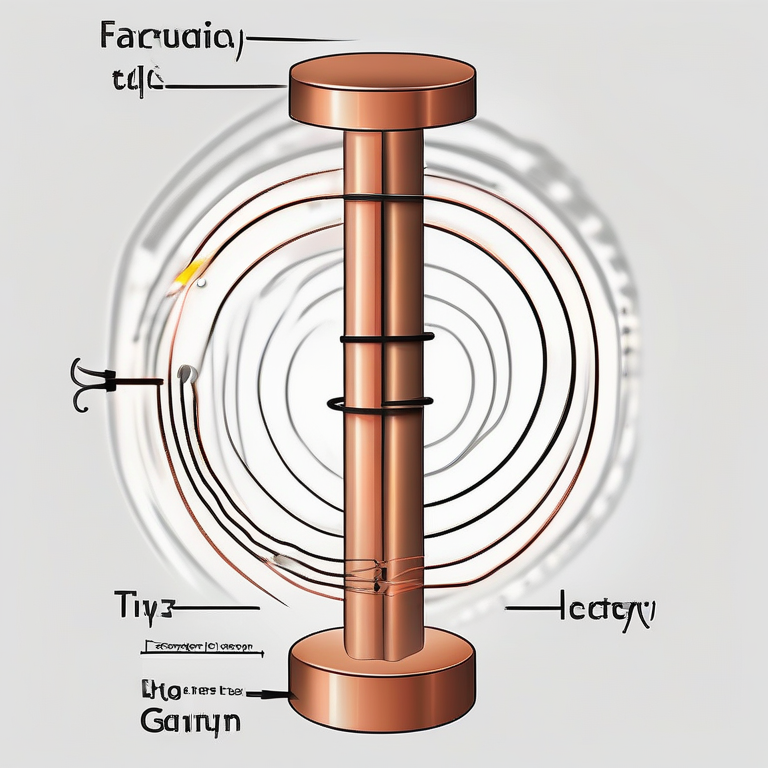
\includegraphics[width=0.6\textwidth]{files/electromagnetism_induction.png}
  \caption{המחשה לחוק פאראדיי: תנועת מגנט ביחס לסליל מוליך משרה זרם חשמלי בסליל.}
\end{figure}

\begin{exampleBox}{דוגמה: כא"מ מושרה בסליל}
סליל בעל 100 ליפופים ממוקם בשדה מגנטי אחיד שניצב למישור הסליל. עוצמת השדה המגנטי משתנה בזמן לפי \(B(t) = 0.1t \, \text{T}\) (טסלה), כאשר \(t\) בזמן (שניות). שטח כל ליפוף בסליל הוא \(0.02 \, \text{m}^2\). מהו הכא"מ המושרה בסליל?

השטף המגנטי דרך ליפוף יחיד הוא \(\Phi_{B, \text{single}} = B \cdot A \cdot \cos\theta\). מכיוון שהשדה ניצב למישור הסליל, הזווית \(\theta = 0\), ו-\(\cos\theta = 1\).
\(\Phi_{B, \text{single}}(t) = B(t) \cdot A = (0.1t) \cdot (0.02) = 0.002t \, \text{Wb}\) (ובר).
השטף הכולל דרך סליל בעל \(N\) ליפופים הוא \(\Phi_B = N \cdot \Phi_{B, \text{single}}\).
כאן \(N = 100\), לכן \(\Phi_B(t) = 100 \cdot (0.002t) = 0.2t \, \text{Wb}\).

לפי חוק פאראדיי, הכא"מ המושרה הוא \(\mathcal{E} = - \frac{d\Phi_B}{dt}\).
נחשב את הנגזרת של השטף הכולל לפי הזמן:
\[\frac{d\Phi_B}{dt} = \frac{d}{dt}(0.2t) = 0.2 \, \text{Wb}/\text{s}\]
\[\frac{d\Phi_B}{dt} = 0.2 \, \text{V}\]
ולכן, הכא"מ המושרה הוא:
\[\mathcal{E} = -0.2 \, \text{V}\]
גודל הכא"מ המושרה הוא \(0.2\) וולט. הסימן השלילי מצביע על כיוון הכא"מ המושרה בהתאם לכלל לנץ. במקרה זה, מכיוון שהשדה גדל עם הזמן, הזרם המושרה (אם המעגל סגור) ייצור שדה מגנטי בכיוון ההפוך לשדה המקורי כדי להתנגד לגידול בשטף.
\end{exampleBox}

סיכום זה מכסה את יסודות החשמל כפי שנדרש. התחום רחב ועמוק בהרבה, אך יסודות אלו מספקים בסיס טוב להמשך לימודים.

\end{document}